% DTMFに関して多少の詳細説明
A watermark of AnnoTone is modulated using DTMF technique mentioned above.
It can contain any kind of annotation data such as integer value, floating-point number, character string, and set of them.
Annotation data is serialized to a byte array and converted to a watermark packet structured as below.

% スペクトログラム
\begin{figure}[htbp]
 \begin{center}
  \includegraphics[width=120mm]{watermarking_spectrogram.png}
 \end{center}
 \caption{The signal spectrogram of a watermark packet that contains a geolocation data from GPS sensor.}
 \label{fig:watr_spec}
\end{figure}

% データフレームの定義
A data frame is the minimum unit of data representation in the watermarking scheme, and is a DTMF signal composed from two sinusoidal waves of the seven sub-carrier frequencies with length of 10 ms.
Since each data frame represents 4-bits information from 0 to 15, a data of one byte is encoded into two data frames.
The former frame represents the lower four bits and the latter represents the higher four bits of a byte.

% パケット模式図
\begin{figure}[htbp]
 \begin{center}
  \vspace{5mm}
  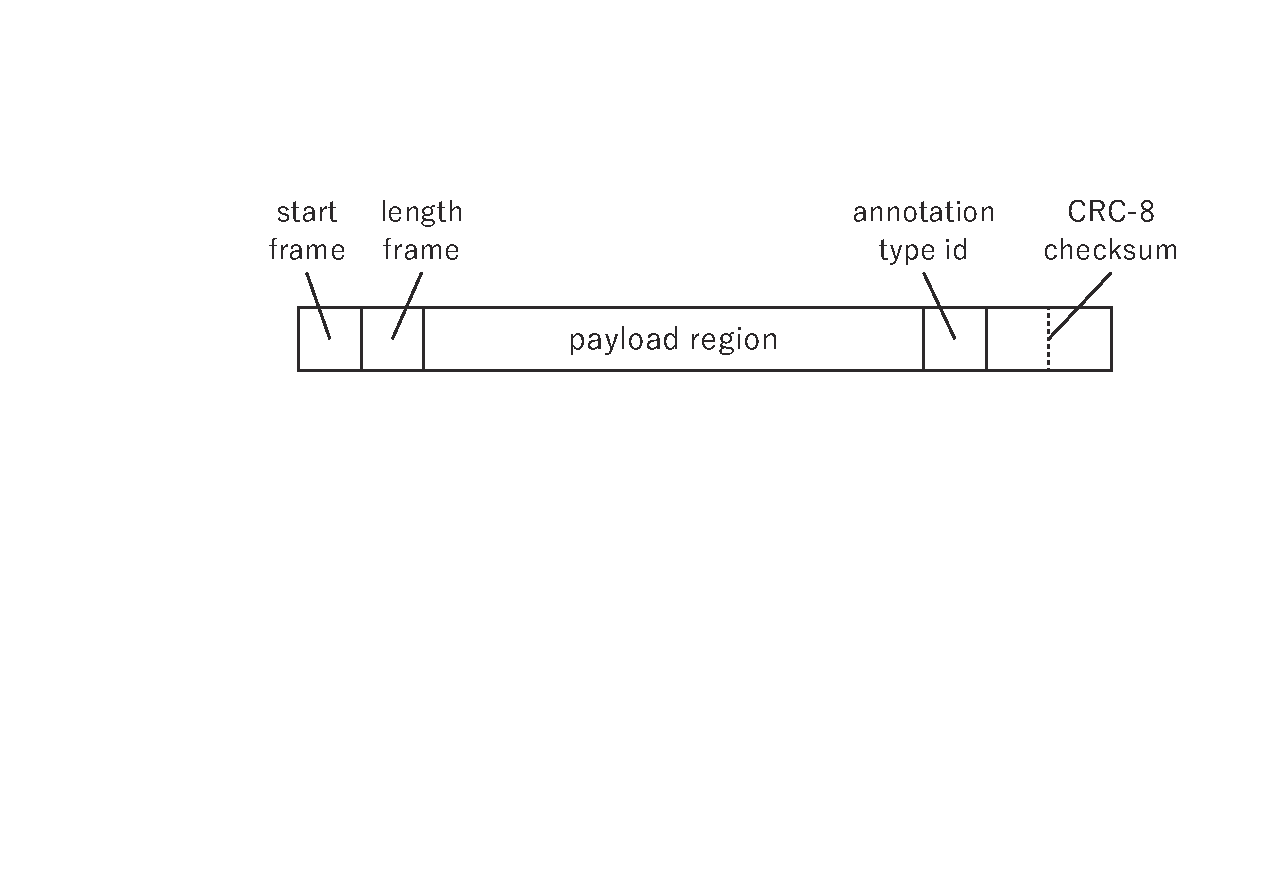
\includegraphics[width=120mm]{watermarking_packet.pdf}
 \end{center}
 \caption{Packet structure.}
 \label{fig:watr_pack}
\end{figure}

% パケットの定義
A packet is a set of several successive data frames representing an annotation data.
The data frame at the head of a packet is called start frame. It is fixed to represent ``2'', and it functions only as a sign of the start position of the packet. There is no special reason for choosing this number.
The second data frame specifies the length of payload region following it to be $ 2^n $ bytes where $n$ is the value of this data frame. It enables a payload size to vary depending on the type of an annotation. Consequently, the size of a packet can also vary.
From the third data frame, a payload region containing the body of an annotation data starts and continues for the length specified in the second data frame.
Multi-byte data such as integer values are ordered in little endian, and multiple data are arranged in their original order in a payload region.
For example, an array of two short integer values \{0x1234, 0x5678\} would be arranged in a payload region as \{4, 3, 2, 1, 8, 7, 6, 5\}.
The data frame after the end of a payload region represents the annotation type id from 0 to 15 to distinguish multiple kinds of annotations embedded in one media file.
An annotation type id for a watermark can be decided arbitrarily by annotating applications.
A packet ends with two data frames representing the CRC-8 checksum of the packet for error detection in decoding. The polynomial for calculating CRC-8 checksum is $x^8 + x^7 + x^6 + x^4 + x^2 + 1$.
